\documentclass[11pt]{article}
\usepackage[T1]{fontenc}
\usepackage{amsmath,amssymb,amsthm}
\usepackage{booktabs}
\usepackage{graphicx}
\usepackage[margin=1in]{geometry}
\usepackage{microtype}
\usepackage{xcolor}
\usepackage[hidelinks]{hyperref}

\definecolor{statusblue}{RGB}{24,72,115}
\newtheorem{theorem}{Theorem}
\newcommand{\symmod}[1]{\left|#1\right|_{\mathrm{sym}}}
\newcommand{\opnorm}[1]{\left\lVert#1\right\rVert_{\infty}}

\title{The sharp $\sqrt2$ constant for the operator symmetric modulus\\
\large Literature-status note for arXiv:2602.19607}
\author{Automated Math Discovery Run \texttt{fa\_banach\_001}, lane 2}
\date{11 August 2026}

\begin{document}
\maketitle

\begin{center}
\fcolorbox{statusblue}{statusblue!6}{\parbox{0.88\linewidth}{
\textbf{Classification: literature already answered.}
The exact construction found independently in this lane appears in Teng Zhang's later paper arXiv:2603.01046. It is recorded here as a verified rediscovery, not as a new result.
}}
\end{center}

\section{Question and disposition}

For a matrix $Z$, write
\[
  \symmod{Z}:=\frac{|Z|+|Z^*|}{2}.
\]
Bourin and Lee prove eigenvalue and symmetric-norm inequalities with constant $\sqrt2$ and ask whether this constant is optimal. The source question is reproduced below from arXiv:2602.19607, PDF page 4.

\begin{center}
  
\includegraphics[width=0.96\linewidth]{figures/open_problem_crop.png}
\end{center}

Teng Zhang's arXiv:2603.01046, submitted six days later, explicitly repeats the question and states that it is answered affirmatively for all $n\geq3$; see the following crop from PDF page 9.

\begin{center}
  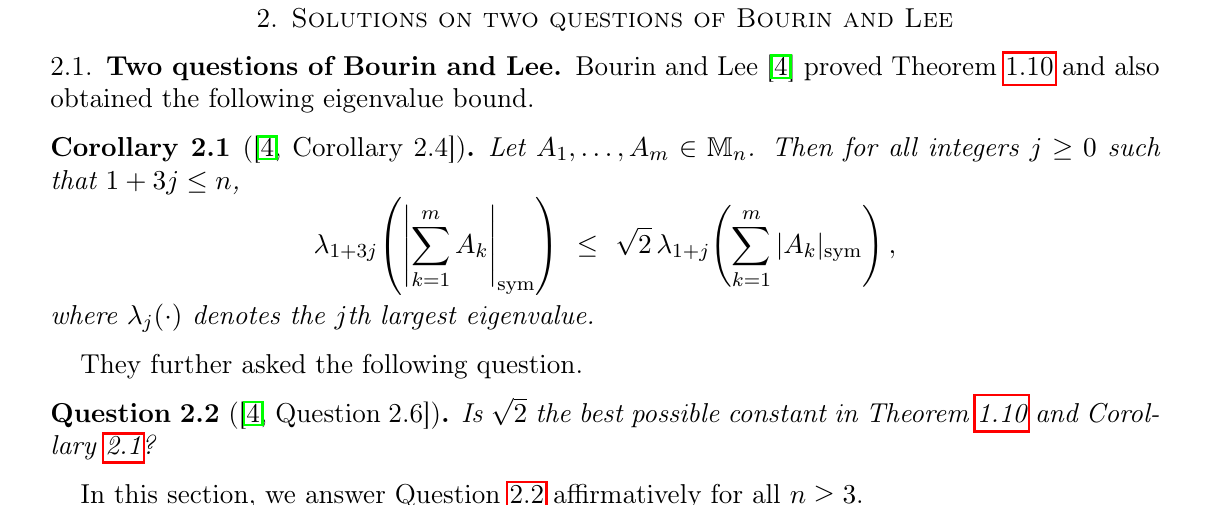
\includegraphics[width=0.96\linewidth]{figures/later_answer_question_crop.png}
\end{center}

\section{Proof intuition}

For a rank-one matrix $R=uv^*$ with unit vectors $u,v$, the two moduli are the endpoint projections: $|R|=vv^*$ and $|R^*|=uu^*$. Thus $\symmod{R}$ is half the sum of two rank-one projections. Four tetrahedral directions in $\mathbb R^3$ form a tight frame, making the denominator exactly scalar. Pairing the directions into two rank-one matrices can simultaneously make their sum have two equal nonzero singular values; its left and right singular subspaces share a line, creating the extra factor $\sqrt2$ in the numerator.

\begin{theorem}[Zhang, arXiv:2603.01046, Theorem 2.5]
The constant $\sqrt2$ in the Bourin--Lee symmetric-norm inequality is optimal for every $n\geq3$. The same example proves optimality in the eigenvalue inequality by taking $j=0$.
\end{theorem}

\begin{proof}[Exact verification]
Work over $\mathbb R^3$ and set
\[
u=\frac1{\sqrt3}\begin{pmatrix}1\\1\\1\end{pmatrix},\quad
v=\frac1{\sqrt3}\begin{pmatrix}1\\-1\\-1\end{pmatrix},\quad
x=\frac1{\sqrt3}\begin{pmatrix}-1\\1\\-1\end{pmatrix},\quad
y=\frac1{\sqrt3}\begin{pmatrix}1\\1\\-1\end{pmatrix}.
\]
Define $A=uv^{\mathsf T}$ and $B=xy^{\mathsf T}$. For unit vectors $a,b$,
\[
 |ab^{\mathsf T}|=bb^{\mathsf T},\qquad
 |(ab^{\mathsf T})^{\mathsf T}|=aa^{\mathsf T},
\]
so
\[
 \symmod{A}+\symmod{B}
 =\frac12(uu^{\mathsf T}+vv^{\mathsf T}+xx^{\mathsf T}+yy^{\mathsf T})
 =\frac23 I_3.
\]
Consequently
\begin{equation}\label{eq:denominator}
 \opnorm{\symmod{A}+\symmod{B}}=\frac23.
\end{equation}

The sum is
\[
S:=A+B=\frac13
\begin{pmatrix}
0&-2&0\\
2&0&-2\\
0&-2&0
\end{pmatrix}.
\]
A direct multiplication gives
\[
S^{\mathsf T}S=\frac19
\begin{pmatrix}4&0&-4\\0&8&0\\-4&0&4\end{pmatrix},\qquad
SS^{\mathsf T}=\frac19
\begin{pmatrix}4&0&4\\0&8&0\\4&0&4\end{pmatrix}.
\]
Each has spectrum $\{8/9,8/9,0\}$ and is $8/9$ times its range projection. Hence
\[
 |S|=\frac{3\sqrt2}{4}S^{\mathsf T}S,\qquad
 |S^{\mathsf T}|=\frac{3\sqrt2}{4}SS^{\mathsf T},
\]
and therefore
\[
 \symmod{S}
 =\frac{3\sqrt2}{8}(S^{\mathsf T}S+SS^{\mathsf T})
 =\operatorname{diag}\!\left(\frac{\sqrt2}{3},\frac{2\sqrt2}{3},\frac{\sqrt2}{3}\right).
\]
Thus
\begin{equation}\label{eq:numerator}
 \opnorm{\symmod{A+B}}=\frac{2\sqrt2}{3}.
\end{equation}
Dividing \eqref{eq:numerator} by \eqref{eq:denominator} gives exactly $\sqrt2$. Since the operator norm is a symmetric norm, no smaller universal constant is possible. For the eigenvalue inequality, $j=0$ reads precisely the same top-eigenvalue/operator-norm estimate. Direct sums $A\oplus0_{n-3}$ and $B\oplus0_{n-3}$ give the result for every $n>3$.
\end{proof}

\section{Match to the independent lane search}

The lane's rank-one optimizer converged to four unoriented tetrahedral lines and produced matrices whose sum is the negative of the displayed $S$, up to relabelling. A global sign does not change $|S|$ or $|S^*|$, so the constructions are mathematically identical. This close match is stronger than merely finding a later theorem with the same conclusion: it shows that the purported new proof route had already been written down in essentially the same form.

The later paper's theorem and calculation are reproduced below from PDF page 10 for auditability.

\begin{center}
  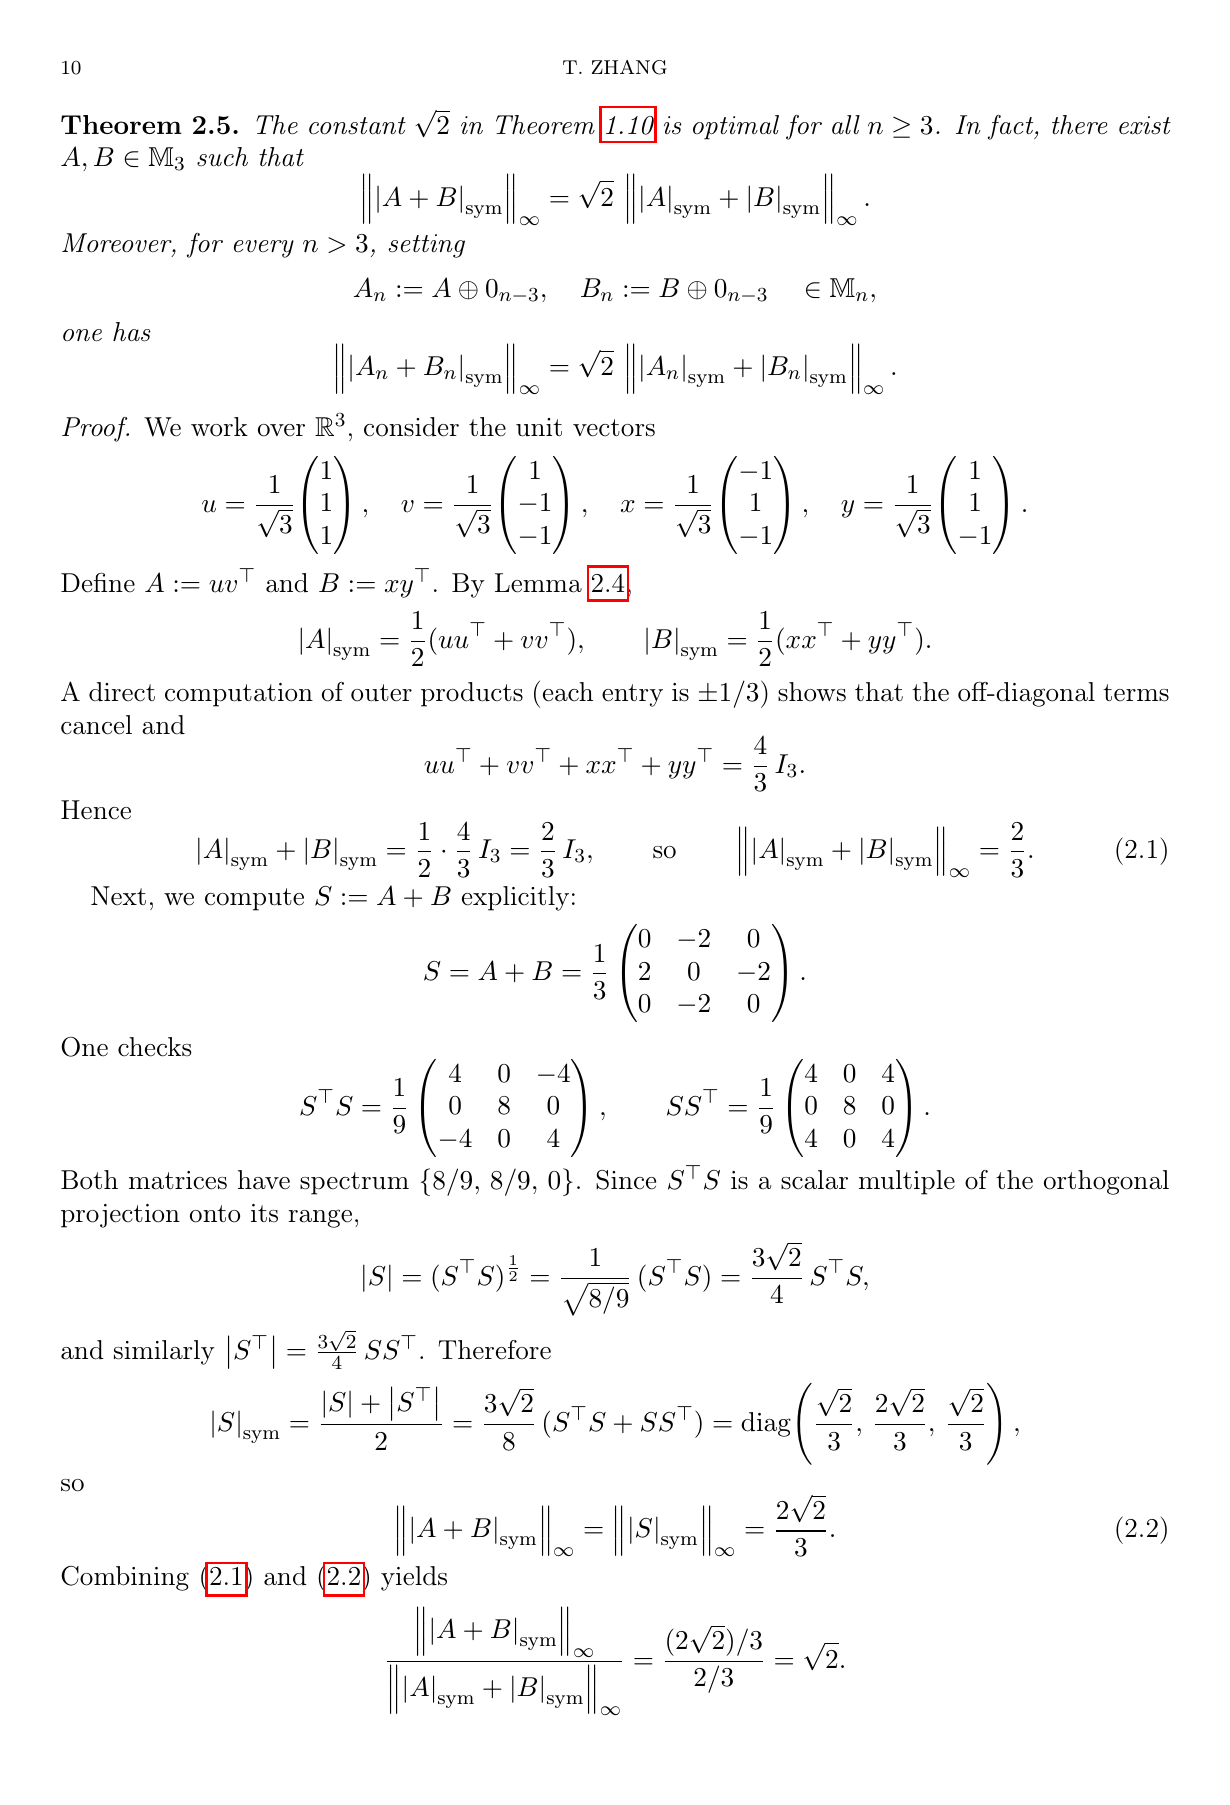
\includegraphics[width=0.92\linewidth]{figures/later_answer_theorem_crop.png}
\end{center}

\section{Scope and conclusion}

The optimality question in arXiv:2602.19607 is fully answered in the later literature. This packet does not claim novelty. The dimension-two optimal constant remains a separate question in Zhang's paper and is outside the source question's universal-constant formulation.

\begin{thebibliography}{9}
\bibitem{BL}
J.-C. Bourin and E.-Y. Lee,
\emph{Triangle inequalities for the operator symmetric modulus},
arXiv:2602.19607 (2026),
\url{https://arxiv.org/abs/2602.19607}.

\bibitem{Z}
T. Zhang,
\emph{Operator symmetric moduli and sharp triangle inequalities},
arXiv:2603.01046 (2026),
\url{https://arxiv.org/abs/2603.01046}.
\end{thebibliography}

\end{document}
